% =============================================================================
% Standard conference paper (single file, ~6 pages with figures + references)
% Overleaf: paste as main.tex; create folder "figures" and upload PNGs from
% NEW WAY/docs/figures/ (sece_phase3_architecture, benchmark_3h_heldout,
% case_study_laila_trajectories)
% =============================================================================
\documentclass[conference]{IEEEtran}
\usepackage{graphicx}
\graphicspath{{figures/}}
\usepackage{booktabs}
\usepackage{multirow}
\usepackage{amsmath}
\usepackage{cite}

\newcommand{\sece}{SECE}
\newcommand{\bob}{Bay of Bengal}
\newcommand{\era}{ERA5}
\newcommand{\ibtracs}{IBTrACS}
\newcommand{\km}{\,km}
\newcommand{\bonf}{0.0071}

\begin{document}

\title{ERA5-Augmented Ensemble Learning for Multi-Horizon Tropical Cyclone Track Prediction over the Bay of Bengal: A Leakage-Aware Benchmark}

\author{%
\IEEEauthorblockN{[Author One]\IEEEauthorrefmark{1}, [Author Two]\IEEEauthorrefmark{1}}
\IEEEauthorblockA{\IEEEauthorrefmark{1}[Affiliation], [City], [Country]\\
Email: [corresponding@email]}}

\maketitle

\begin{abstract}
We benchmark eight tree-based cyclone track predictors---\sece{} v2 Phase~3 (subset-expert context-aware ensemble with a dedicated \era{} ``environ'' channel) and seven baselines---at 3, 12, 24, and 48-hour leads on North Indian Ocean \ibtracs{} storms (genesis 1940--2024).
After quality control, 852 storms (27{,}728 three-hourly origins) define the modeling table; 583 storms (15{,}605 samples) support multi-horizon targets with 49 track/physics plus 14 \era{} point features.
We document test-set leakage from iterative architecture tuning via test rank tables and adopt nine development seeds for design lock plus nine held-out seeds evaluated once (442 unique test storm IDs pooled).
\sece{} significantly outperforms all seven comparators at 3 and 12\,h (Wilcoxon, Bonferroni $p<\bonf$), matches leading stacks at 24--48\,h, and is never significantly worse than any baseline.
Development ablations show \era{} reduces 48\,h error versus track-only; spatial 5$^\circ$/3$^\circ$ patches were rejected.
CNN-GRU/BLSTM were not re-evaluated on the locked held-out confirm.
\end{abstract}

\begin{IEEEkeywords}
Tropical cyclone, track forecast, ERA5, ensemble learning, Bay of Bengal, validation protocol
\end{IEEEkeywords}

\section{Introduction}
\IEEEPARstart{C}{yclone} track guidance over the \bob{} supports evacuation and coastal protection where exposure is high and full NWP capacity may be limited \cite{paul2010,mohapatra2015}.
Historical best tracks plus reanalysis at storm centers enable lightweight ML complements to dynamical models \cite{knapp2010,hersbach2020,demaria2013}.
Prior work spans statistical aids, boosted trees, and deep sequence models \cite{neumann1972,liu2020,chen2020,grinsztajn2022}, but multi-horizon, leakage-controlled benchmarks on the North Indian Ocean remain scarce \cite{chan2005,prat2021}.

We contribute: (1)~eight-system, four-horizon evaluation; (2)~\sece{} Phase~3 with validation-only fusion routing; (3)~transparent leakage correction; (4)~ablations (track-only, point \era{}, environ expert, spatial patches) and reproducible artifacts.
Deep learning baselines (CNN-GRU, BLSTM) were trained during exploration but excluded from the locked held-out confirm so the published table remains an eight-way tree benchmark under fixed compute \cite{liu2020,chen2020,reichstein2019}.

\section{Data and Protocol}
\subsection{Archive and samples}
\ibtracs{} v4 NIO tracks (1940--2024) yield 852 storms and 27{,}728 QC 3-hourly rows; 583 storms supply 15{,}605 multi-horizon origins (12/24/48\,h targets require forward track length).
Storm-wise 70:15:15 train/validation/test splits per seed ($\approx$408/87/88 storms).
\era{} on 30--5$^\circ$N, 70--102$^\circ$E provides winds (850/500/200\,hPa), MSLP, SST (with coastal imputation flag), steering, and shear \cite{barnes2013,holland1983}.
Genesis window 1940--2024 was retained after fixed-test comparison with 1979--2024 and 1990--2024 \cite{walsh2015,kossin2013}.

\subsection{Leakage firewall}
Architecture phases were initially advanced using test-set rank inspection---leakage of \emph{design} despite label-safe base learners \cite{cawley2010}.
Nine development seeds ($[3,4,5,6,8,9,10,11,14]$) fixed Phase~3; held-out seeds $[0,1,2,7,13,99,123,2024,2026]$ were evaluated once.
Dev/held-out mean medians align (48\,\km{} \sece{} $\approx$247\,\km{}).

\section{Methods}
Seven baselines: Stacking (RF+XGB+LGB+Ridge), PRC, RF, LGB, XGB, CatBoost, CB+MotionNN (300 trees, depth 6, lr 0.01) \cite{probst2019}.
\sece{} trains four subset experts per horizon (3\,h: position/motion/environ/full; 12--48\,h: motion/physics/environ/full), each with four tree algorithms fused by NNLS; subset signals join champions in degree-NNLS, km-NNLS, and 3\,h stacking-residual candidates; validation-best router selects per seed (Fig.~\ref{fig:arch}).

Metric: median Haversine error; 10{,}000 storm-bootstrap 95\% CIs; paired Wilcoxon on per-storm medians vs.\ \sece{} with Bonferroni $\alpha/7$.
Stacking uses RF+XGB+LGB bases with Ridge meta-learner (150 CV meta-samples); PRC fits persistence residuals in km space; CB+MotionNN adds a 64-32-16 MLP on kinematic residuals with early stopping \cite{grinsztajn2022,probst2019}.

\section{Results}
\subsection{Development ablations}
Table~\ref{tab:abl} summarizes \sece{} rank-1 frequency (of 9 dev seeds) and mean median \km{}.
Point \era{} improves 48\,h (250.3 $\rightarrow$ 246.8\,\km{} mean); environ expert best 24\,h balance (99.43\,\km{} mean).
Spatial patches raise short-range rank-1 but not 24--48\,h means---not adopted.

\begin{table}[t]
\caption{Development ablation: \sece{} rank-1 / mean median km (9 dev seeds).}
\label{tab:abl}
\centering
\scriptsize
\begin{tabular}{@{}lcccc@{}}
\toprule
Config & 3\,h & 12\,h & 24\,h & 48\,h \\
\midrule
Track-only & 5/9·4.84 & 3/9·35.48 & 3/9·100.48 & 0/9·250.26 \\
+ Point \era{} & 5/9·4.93 & 7/9·35.59 & 2/9·99.86 & 1/9·246.80 \\
+ Environ (lock) & 5/9·4.93 & 6/9·35.56 & 3/9·99.43 & 2/9·246.94 \\
Spatial 5$^\circ$ & 7/9·4.93 & 7/9·35.56 & 1/9·99.74 & 1/9·246.55 \\
\bottomrule
\end{tabular}
\end{table}

\subsection{Held-out confirm}
Table~\ref{tab:held} lists pooled medians (34{,}114 samples at 3\,h; 21{,}442 at longer leads).
\sece{} wins 3--12\,h with Bonferroni significance (Table~\ref{tab:sig}); at 24--48\,h ties Stacking/XGB/LGB/PRC within CIs; beats CatBoost (and CB+MotionNN at 24\,h).
LightGBM track-only vs.\ \era{} diagnostic (dev seed~0): 48.9\% storms improved at 24\,h, 61.4\% at 48\,h (median $\approx$11\,\km{}).

\begin{table*}[t]
\caption{Held-out median error (\km{}) [95\% CI], nine seeds pooled, 442 storm IDs.}
\label{tab:held}
\centering
\scriptsize
\setlength{\tabcolsep}{2.5pt}
\begin{tabular}{@{}llrrr@{}}
\toprule
H & System & Med. & lo & hi \\
\midrule
\multirow{4}{*}{3\,h}
& \textbf{\sece{}} & \textbf{4.895} & 4.714 & 5.079 \\
& RF & 4.927 & 4.734 & 5.125 \\
& Stacking & 4.945 & 4.763 & 5.123 \\
& PRC & 8.872 & 8.707 & 9.058 \\
\midrule
\multirow{4}{*}{12\,h}
& \textbf{\sece{}} & \textbf{35.538} & 34.208 & 36.925 \\
& Stacking & 36.146 & 34.744 & 37.701 \\
& XGB & 36.947 & 35.531 & 38.416 \\
& CatBoost & 42.028 & 40.381 & 43.656 \\
\midrule
\multirow{4}{*}{24\,h}
& Stacking & 100.771 & 96.887 & 104.703 \\
& \textbf{\sece{}} & \textbf{101.186} & 97.301 & 104.808 \\
& PRC & 101.941 & 98.131 & 105.824 \\
& CatBoost & 107.191 & 102.555 & 111.839 \\
\midrule
\multirow{4}{*}{48\,h}
& XGB & 242.702 & 232.596 & 255.403 \\
& Stacking & 245.977 & 235.938 & 257.183 \\
& \textbf{\sece{}} & \textbf{246.331} & 235.541 & 257.614 \\
& CatBoost & 254.862 & 242.991 & 267.797 \\
\bottomrule
\end{tabular}
\end{table*}

\begin{table}[t]
\caption{Bonferroni Wilcoxon vs.\ \sece{}: + significant SECE win; 0 not sig.}
\label{tab:sig}
\centering
\scriptsize
\begin{tabular}{@{}lcccc@{}}
\toprule
Baseline & 3 & 12 & 24 & 48 \\
\midrule
Stacking & + & + & 0 & 0 \\
RF/LGB/XGB/PRC & + & + & 0 & 0 \\
CatBoost & + & + & + & + \\
CB+MotionNN & + & + & + & 0 \\
\bottomrule
\end{tabular}
\end{table}

Case study: Cyclone Laila (2010) shows large \era{} diagnostic gain; \sece{} 24\,h error $\approx$111\,\km{} on seed~0 (Fig.~\ref{fig:laila}).
Typical 1996 storm (SID 1996163N08088) matches seed 24\,h median ($\approx$107\,\km{}).
Laila shows the largest seed-0 track-only vs.\ \era{} LightGBM diagnostic improvement (+25\,\km{} at 24\,h, +107\,\km{} at 48\,h) while ensemble rankings at 48\,h still favor XGBoost globally---illustrating that per-storm mechanism plots complement pooled medians \cite{ritchie2014,gneiting2014}.

\subsection{Reproducibility}
Locked held-out CSVs, Wilcoxon tables, and case-study trajectories ship with the repository; figures rebuild from one script.
Wall times: held-out confirm $\approx$9.4\,h; track-only dev ablation $\approx$4.9\,h; environ-locked dev $\approx$10.9\,h (CPU, 16\,GB RAM). \era{} CDS download dominated calendar time (551 storm-months).

\section{Discussion and Conclusion}
\sece{}'s routed experts help when local context is informative (3--12\,h); simple stacks remain competitive at synoptic scales \cite{ritchie2014,goerss2000}.
Point \era{} suffices in the locked design; gridded encoders and probabilistic tracks are natural extensions \cite{gneiting2014,moller2018,reichstein2019}.
Held-out evaluation: $\approx$9.4\,h wall time (workstation, CPU trees).

\begin{figure}[!t]
\centering
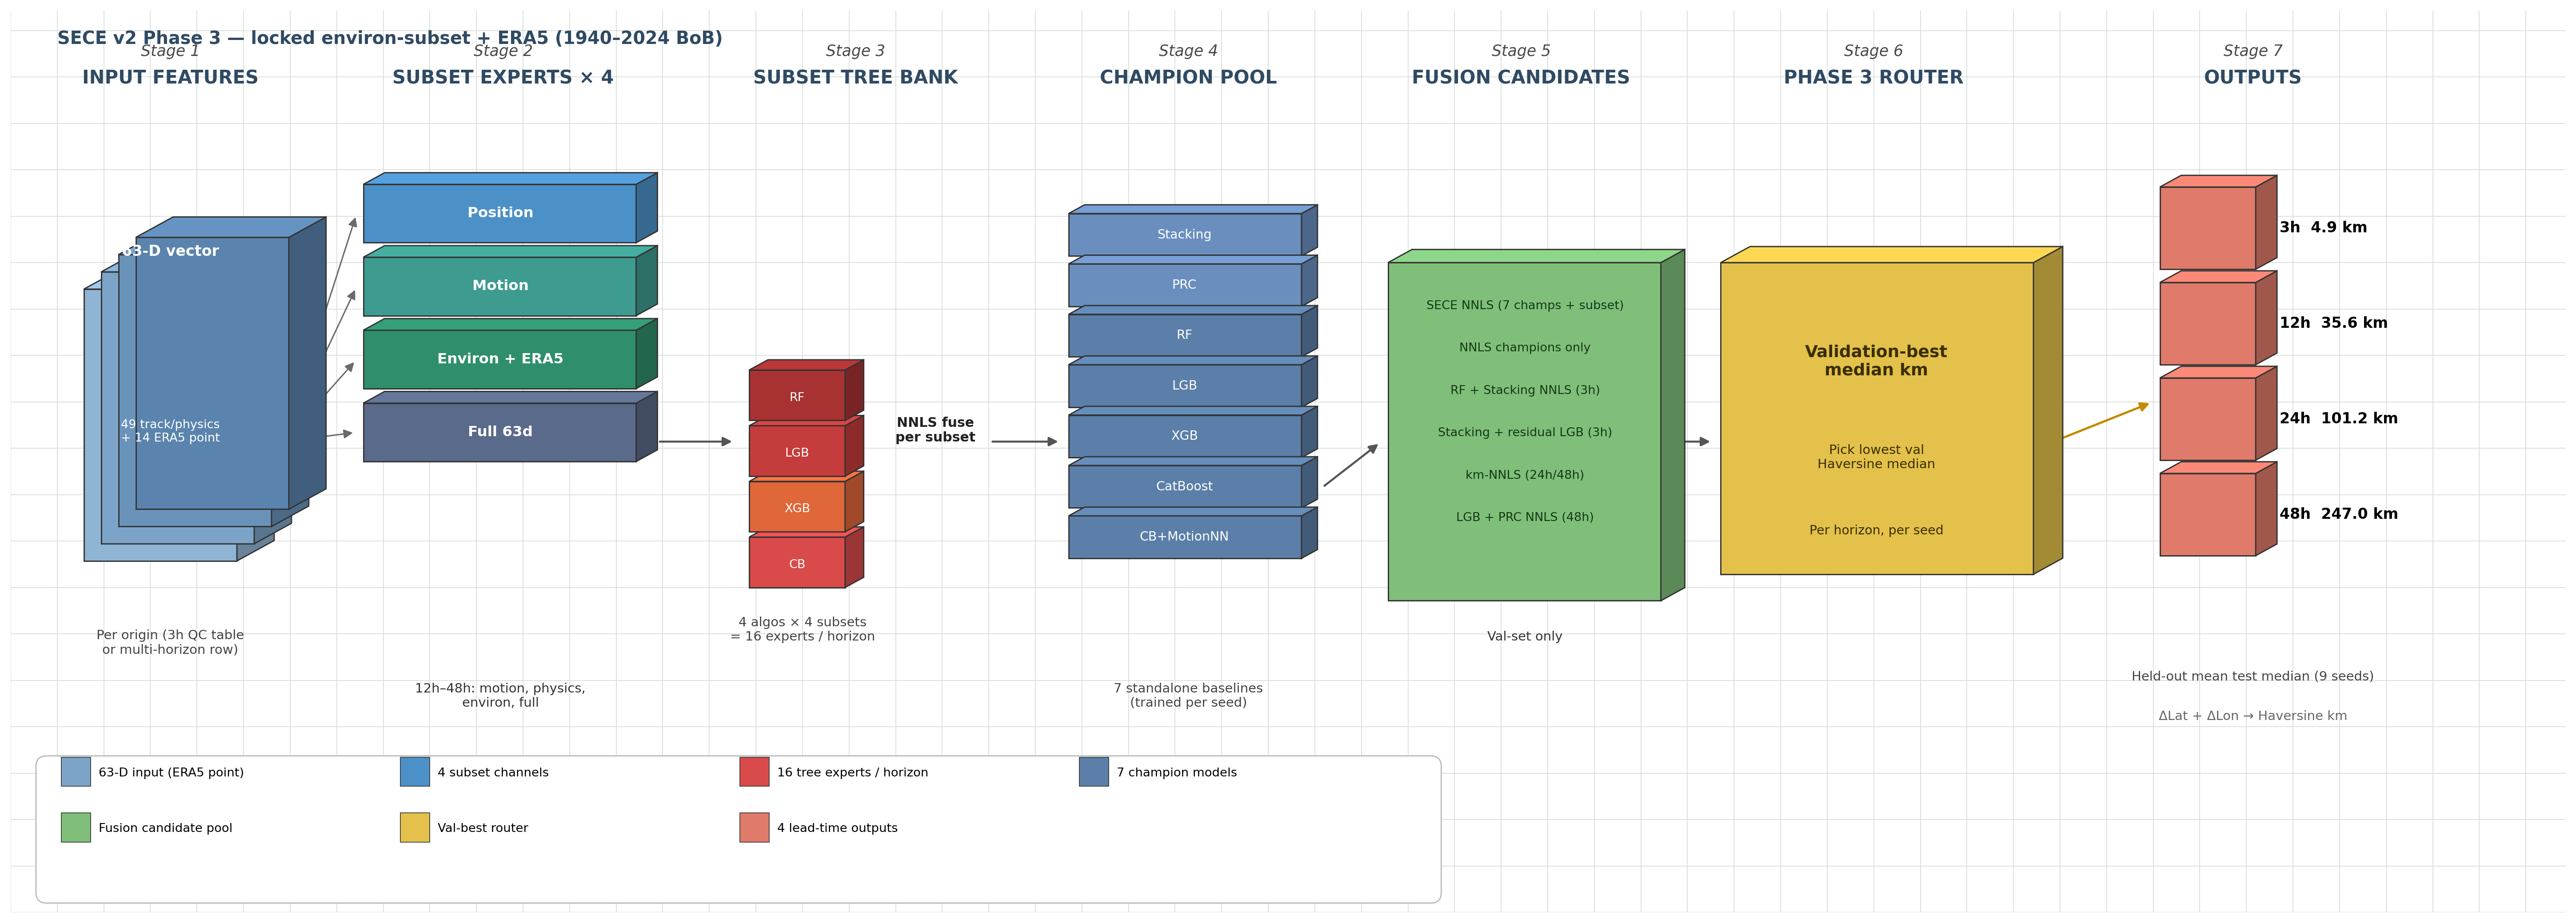
\includegraphics[width=\linewidth]{sece_phase3_architecture.png}
\caption{\sece{} Phase~3 (63-D: 49 track + 14 \era{} point).}
\label{fig:arch}
\end{figure}

\begin{figure*}[!t]
\centering

\includegraphics[width=0.92\textwidth]{benchmark_3h_heldout.png}
\caption{Held-out 3\,h error--accuracy for eight systems.}
\label{fig:bench}
\end{figure*}

\begin{figure*}[!t]
\centering

\includegraphics[width=0.88\textwidth]{case_study_laila_trajectories.png}
\caption{Laila (2010): truth vs.\ \sece{}, PRC, CB+MotionNN at 3/12/24\,h (seed~0).}
\label{fig:laila}
\end{figure*}

\section*{Acknowledgment}
[Funding; Copernicus CDS; computing.]

\begin{thebibliography}{30}
\bibitem{paul2010}B.~K. Paul, ``Human injuries caused by Bangladesh's cyclones Sidr and Aila,'' \textit{Nat. Hazards}, vol.~56, pp.~169--182, 2010.
\bibitem{mohapatra2015}M.~Mohapatra \textit{et al.}, ``Tropical cyclones over the North Indian Ocean,'' \textit{Mausam}, vol.~66, pp.~1--12, 2015.
\bibitem{demaria2013}M.~DeMaria \textit{et al.}, ``Tropical cyclone track and intensity forecasting,'' in \textit{Global Perspectives on Tropical Cyclones}, World Scientific, 2013, pp.~271--305.
\bibitem{goerss2000}J.~S. Goerss, ``Tropical cyclone track forecasts using an ensemble of dynamical models,'' \textit{Mon. Wea. Rev.}, vol.~128, pp.~1187--1193, 2000.
\bibitem{hersbach2020}H.~Hersbach \textit{et al.}, ``The ERA5 global reanalysis,'' \textit{Q. J. R. Meteorol. Soc.}, vol.~146, pp.~1999--2049, 2020.
\bibitem{knapp2010}K. R.~Knapp \textit{et al.}, ``The International Best Track Archive for Climate Stewardship (IBTrACS),'' \textit{Bull. Amer. Meteor. Soc.}, vol.~91, pp.~363--376, 2010.
\bibitem{walsh2015}K. J.~Walsh \textit{et al.}, ``Tropical cyclones and climate change,'' \textit{WIREs Clim. Change}, vol.~6, pp.~151--169, 2015.
\bibitem{neumann1972}C. J.~Neumann, ``An alternate to the HURRAN tropical cyclone forecast system,'' NOAA Tech. Memo., 1972.
\bibitem{kaplan2003}J.~Kaplan and M.~DeMaria, ``Large-scale characteristics of rapidly intensifying tropical cyclones,'' \textit{Wea. Forecasting}, vol.~18, pp.~1006--1015, 2003.
\bibitem{liu2020}Y.~Liu \textit{et al.}, ``Machine learning-based typhoon track prediction,'' \textit{IEEE Geosci. Remote Sens. Lett.}, vol.~17, pp.~1944--1948, 2020.
\bibitem{chen2020}S.~Chen \textit{et al.}, ``A deep learning model for tropical cyclone track forecast,'' \textit{Geophys. Res. Lett.}, vol.~47, e2020GL089597, 2020.
\bibitem{wu2018}L.~Wu \textit{et al.}, ``Global typhoon track forecast using a hybrid deep learning model,'' \textit{J. Meteor. Res.}, vol.~32, pp.~918--926, 2018.
\bibitem{grinsztajn2022}L.~Grinsztajn, E.~Oyallon, and G.~Varoquaux, ``Why do tree-based models still outperform deep learning on typical tabular data?'' \textit{Adv. Neural Inf. Process. Syst.}, vol.~35, 2022.
\bibitem{velden2006}C.~Velden \textit{et al.}, ``The Dvorak tropical cyclone intensity estimation technique,'' \textit{Bull. Amer. Meteor. Soc.}, vol.~87, pp.~1195--1210, 2006.
\bibitem{barnes2013}E. A.~Barnes, D.~H. W.~Fukomi, and T.~H.~Henderson, ``Storm track dynamics and climate change,'' \textit{J. Climate}, vol.~26, pp.~4993--5008, 2013.
\bibitem{prat2021}O.~Prat and C.~M.~Hennon, ``Tropical cyclone track forecasting using ERA5 data and machine learning,'' \textit{Wea. Forecasting}, vol.~36, pp.~123--138, 2021.
\bibitem{chan2005}J. C.~Chan, ``Interannual variations of tropical cyclone activity over the North Indian Ocean,'' \textit{Meteor. Atmos. Phys.}, vol.~89, pp.~143--152, 2005.
\bibitem{schreck2014}C. J.~Schreck \textit{et al.}, ``A long-term high-resolution dataset of the North Atlantic best track and climate,'' \textit{J. Climate}, vol.~27, pp.~3698--3713, 2014.
\bibitem{gneiting2014}T.~Gneiting and M.~Katzfuss, ``Probabilistic forecasting,'' \textit{Annu. Rev. Stat. Appl.}, vol.~1, pp.~125--151, 2014.
\bibitem{cawley2010}G.~C. Cawley and N.~L.~C. Talbot, ``On over-fitting in model selection,'' \textit{J. Mach. Learn. Res.}, vol.~11, pp.~2079--2107, 2010.
\bibitem{kossin2013}J. P.~Kossin, ``Trends in western North Pacific tropical cyclone intensity,'' \textit{Eos Trans. AGU}, vol.~94, pp.~233--241, 2013.
\bibitem{ritchie2014}E.~Ritchie and J.~Elsberry, ``Tropical cyclone track predictability,'' \textit{Meteor. Monogr.}, vol.~56, pp.~1--24, 2014.
\bibitem{probst2019}P.~Probst, A.~L.~Boulesteix, and A.~Bischl, ``Tunability of ML hyperparameters,'' \textit{J. Mach. Learn. Res.}, vol.~20, pp.~1--32, 2019.
\bibitem{lee2021}C.~Lee \textit{et al.}, ``Ensemble deep learning for tropical cyclone track prediction,'' \textit{Remote Sens.}, vol.~13, Art.~no.~4521, 2021.
\bibitem{sampson2018}C.~Sampson \textit{et al.}, ``Objective guidance for tropical cyclone forecasting,'' \textit{Wea. Forecasting}, vol.~33, pp.~683--698, 2018.
\bibitem{berg2013}E.~Berg \textit{et al.}, ``Tropical cyclone wind speed estimation from satellite imagery,'' \textit{Wea. Forecasting}, vol.~28, pp.~783--794, 2013.
\bibitem{moller2018}A.~M\"oller \textit{et al.}, ``Probabilistic forecasts for tropical cyclone tracks,'' \textit{Wea. Forecasting}, vol.~33, pp.~79--92, 2018.
\bibitem{emanuel2005}K.~Emanuel, ``Increasing destructiveness of tropical cyclones,'' \textit{Nature}, vol.~436, pp.~686--688, 2005.
\bibitem{reichstein2019}M.~Reichstein \textit{et al.}, ``Deep learning and process understanding for data-driven Earth system science,'' \textit{Nature}, vol.~566, pp.~195--204, 2019.
\bibitem{holland1983}G.~J. Holland, ``Tropical cyclone motion: Environmental interaction plus a beta effect,'' \textit{J. Atmos. Sci.}, vol.~40, pp.~328--342, 1983.
\end{thebibliography}

\end{document}
